\chapter{Peer-Assisted View-Dependent Streaming}
\label{c:p2p}
\section{Introduction}
    In applications such as virtual art gallery, virtual
    earth, virtual museums, and virtual auction house,
    statues, artifacts, and auction items are streamed to
    potentially a large number of visitors or bidders,
    sometimes within a short period of time (e.g., when an
    item is released for bidding).  The clients for these
    applications are likely to inspect the items carefully,
    zooming in to view the fine details, and rotating the
    item back-and-forth to examine all facets of an item.
    Such flash crowd can potentially impose substantial
    bandwidth requirements on the server.

    Peer-to-peer (P2P) data dissemination is commonly used to
    alleviate server's bandwidth cost.  Downloading
    peers forward the received data to other peers,
    contributing their upload bandwidth and reducing the
    burden of the server, hence allowing more users to
    be supported.  P2P techniques have been successfully used 
    in bulk file transfer (e.g., BitTorrent) and video
    streaming (e.g., PPLive).

    Using P2P techniques for view-dependent progressive mesh
    streaming, or \textit{P2P mesh streaming} for short, poses 
    several new challenges.  First, each
    client may view, and therefore request mesh data, in a 
    different order.
    Thus, a client needs
    to frequently search for peers to download visible mesh
    data from when its view point changes.  Second, we
    found that a user stays in the system for a short time,
    in the order of minutes (See Section \ref{ss:user:session})
    when viewing a mesh, leading to high churn rate.  Third,
    determining the visible region of a mesh given a view
    point is computationally intensive and is
    traditionally done at the server.  In the P2P context,
    how to determine the visible region of a mesh is
    non-trivial.

    Fortunately, the nature of mesh streaming alleviates
    other constraints in the system design:  (i) we found
    that users can tolerate higher response time when
    interacting with the mesh, due to progressive mesh rendering, 
    and (ii) unlike video, there is no strict 
    deadline to render the mesh.
    Together, these differences 
    %in the nature of mesh streaming 
    lead us to new challenges and different design decisions in 
    designing P2P mesh streaming systems, in contrast to P2P
    video streaming and P2P file downloading.  This chapter
    reports on our design of a P2P mesh streaming system and
    its evaluations.

    In P2P data dissemination, the data (a file, video, or
    mesh) are typically divided into \textit{chunks}.  A
    peer that has downloaded a chunk can potentially serve
    this chunk to other peers.  We call such a peer a
    \textit{provider} of the chunk.  This chapter addresses
    two important design questions of P2P mesh streaming.

    The first question is how to define a chunk.  While one 
    can easily segment a 
    file or a video into chunks, due to progressivity
    of progressive meshes, chunks have to be carefully 
    constructed in a hierarchical way that can
    incrementally improve the quality of the mesh, with
    minimal coding dependency among the chunks.
    Moreover, chunk size should be small enough to 
    reduce the fraction of invisible vertex splits
    received. 

    Second, how can
    a peer know the best provider of a given chunk?   
    Consider the a large number of queries and high churn
    rate, we first consider simply using a 
    centralized lookup service for chunk provider,
    allowing fast peer failure detection and one-hop lookup.
    Centralized lookup, however, is not scalable to large
    number of peers, due to the overhead in maintaining
    peer states and handling queries.
    We therefore propose a hierarchical P2P
    system, which retains the advantages of centralized
    lookup but with significantly fewer 
    requests to the server.  The
    basic idea is to group peers according to the
    hierarchical structure of chunks in a progressive mesh.
    Each group has a leader that takes over most of the responsibilities of the server to
    reduce server overhead.
    
    Our contributions in this chapter are as follows.
    First, we compare and contrast P2P mesh streaming to P2P
    video streaming and P2P file downloading and point out
    the main difficulties of P2P mesh streaming.  Second, 
    considering the differences and challenges, 
    we investigate on two content discovery schemes for P2P
    mesh streaming.  The structure of the progressive
    mesh is considered in the second design to further
    reduce server overhead.  Third, we propose a 
    chunking scheme for progressive meshes to support P2P mesh
    streaming.  Finally, we run simulations based on real
    traces collected from users to evaluate the P2P
    mesh streaming system we proposed.  Analysis and
    simulation results show that server overhead can be
    reduced by 90\%. Meanwhile,  average response time and
    control overhead are low.

    We structure the rest of this chapter as follows.  
    %We introduce previous work on progressive mesh streaming
    %and P2P techniques in Section \ref{s:related}.  
    We
    compare P2P mesh streaming with P2P video streaming and
    P2P file downloading in Section \ref{s:comp}.  
    %Sections \ref{s:receiver} and \ref{s:chunk} introduces the
    %receiver-driven protocol and the hierarchical chunk structure,
    Section \ref{s:chunk} introduces the hierarchical chunk structure.
    %two essential components of our system, respectively.  
    We propose two content discovery schemes
    in Section \ref{s:content}, and the experimental results in Section
    \ref{s:experiment}.
    Finally, we conclude in Section \ref{s:conclude}.

%\section{Related Work}
%\label{s:related}
\section{P2P Video Streaming}
\label{ss:related_p2p}
%simplified by Liu Dan
P2P techniques have been widely studied in file downloading, live
streaming, and video-on-demand (VoD) streaming applications. In this section,
we introduce the related work on P2P video streaming systems.

Generally, P2P streaming systems can be categorized into tree-based
and mesh-based approaches. In tree-based approaches, peers are
organized into a single tree \cite{jannotti:overcast, chu:narada}
or multiple trees \cite{castro:splitstream,
padmanabhan:coopnet}.
%Compared to the single-tree structure, multiple-tree topology is more
%robust to node dynamics, more scalable, and also more widely exploited
%in P2P video streaming protocols. 
In typical multi-tree-based
approaches, like CoopNet \cite{padmanabhan:coopnet}, different parts of a video segment are
separately pushed down along different sub-trees. SplitStream
\cite{castro:splitstream}
utilizes Multiple Description Coding (MDC) scheme to further improve
streaming quality by introducing data redundancy. Besides, each peer
serves as an interior node in only one sub-tree to minimize the
negative effect of node failures. 
%Even so, multiple-tree-based
%approaches still have the limitations in terms of robustness and
%scalability.

To further improve robustness and scalability, mesh-based approaches
have been more widely explored in P2P live streaming systems,
including PPLive and PPStream. Typically, gossip-like protocols are
used for peers to pull video content from qualified peers. Compared to
tree-based approaches, such systems incur higher end-to-end latency
and control overhead. To reduce these negative effects,
push-pull-based approaches are proposed in \cite{zhang:coolstreaming}. 
Moreover, PRIME \cite{magharei:prime}
incorporates swarming scheme and MDC to improve robustness and
streaming quality, but its two-phase design increases end-to-end
latency.

Similar tree-based and mesh-based approaches can also be utilized in
P2P VoD streaming. Different from live streaming, peers
may seek to different playback points in the video, causing
higher peer dynamics. 
%Therefore, tree-based approaches, like P2VoD
%\cite{do:p2vod},
% are not good choices for P2P VoD. 
Further, since peers have different views of the video, it is more challenging
to locate providers. The oStream \cite{cui:ostream} system
utilizes sliding window to maintain certain video content so that
peers can obtain content from other peers with smaller interval
between their windows. Yiu et al. \cite{yiu:distributed} propose that
each peer randomly stores some segments and uses DHT to locate peers
storing previous, current, and next segments, respectively. This
approach can achieve better scalability and shorter initial delay than
sliding window scheme, but maintaining the segment
lists in a highly dynamic environment is difficult.
   
\section{P2P Mesh Streaming}
\label{s:comp}

    Although P2P techniques have already been studied in
    file downloading, live video streaming, and
    video-on-demand streaming, P2P view-dependent
    progressive mesh streaming (or P2P mesh streaming for
    short) has a different set of requirements and
    characteristics, leading to different design decisions and
    new challenges.
    In this section, we elaborate on these differences.

    In P2P file sharing, a peer is interested in obtaining a
    complete file.  In most cases, the file is not useful
    until it is completely downloaded.  During downloading,
    \textit{any} new chunk of the file downloaded is useful.
    %A peer is equally likely to have a chunk than any other
    %peers.  
    Chunks can be downloaded in any order.
    Therefore, peer $p$ can receive chunks from peer $q$ as
    long as $q$ possesses fresh chunks that $p$ have
    not received.

    In P2P video streaming, however, the video is played
    back mostly in the increasing time order\footnote{unless the
    user seek to another playback point}.  The point the
    peer is watching the video is the \textit{playback
    time}, and each chunk in the video has an associated
    timestamp.  Unlike file sharing, not every chunk is
    useful.  A peer is only interested in a chunk whose
    timestamp is later than the playback time.  Chunks
    nearer to the playback time have higher priority.  
    %To download a chunk with timestamp $t$, a peer should
    %contact all other peers whose playback time is later
    %than $t$ or close to $t$.  Further, since 
    Since chunks are
    needed and playback in the same order, if a peer $p$
    receives a chunk with timestamp $t$ from a peer $q$, it
    is likely that $p$ can receive the chunk with timestamp
    $t+1$ from $q$.  In other words, a peer can exploit
    \textit{temporal locality} in chunk access to discover
    other peers to retrieve the chunks from.

    \begin{figure}
    \centering
    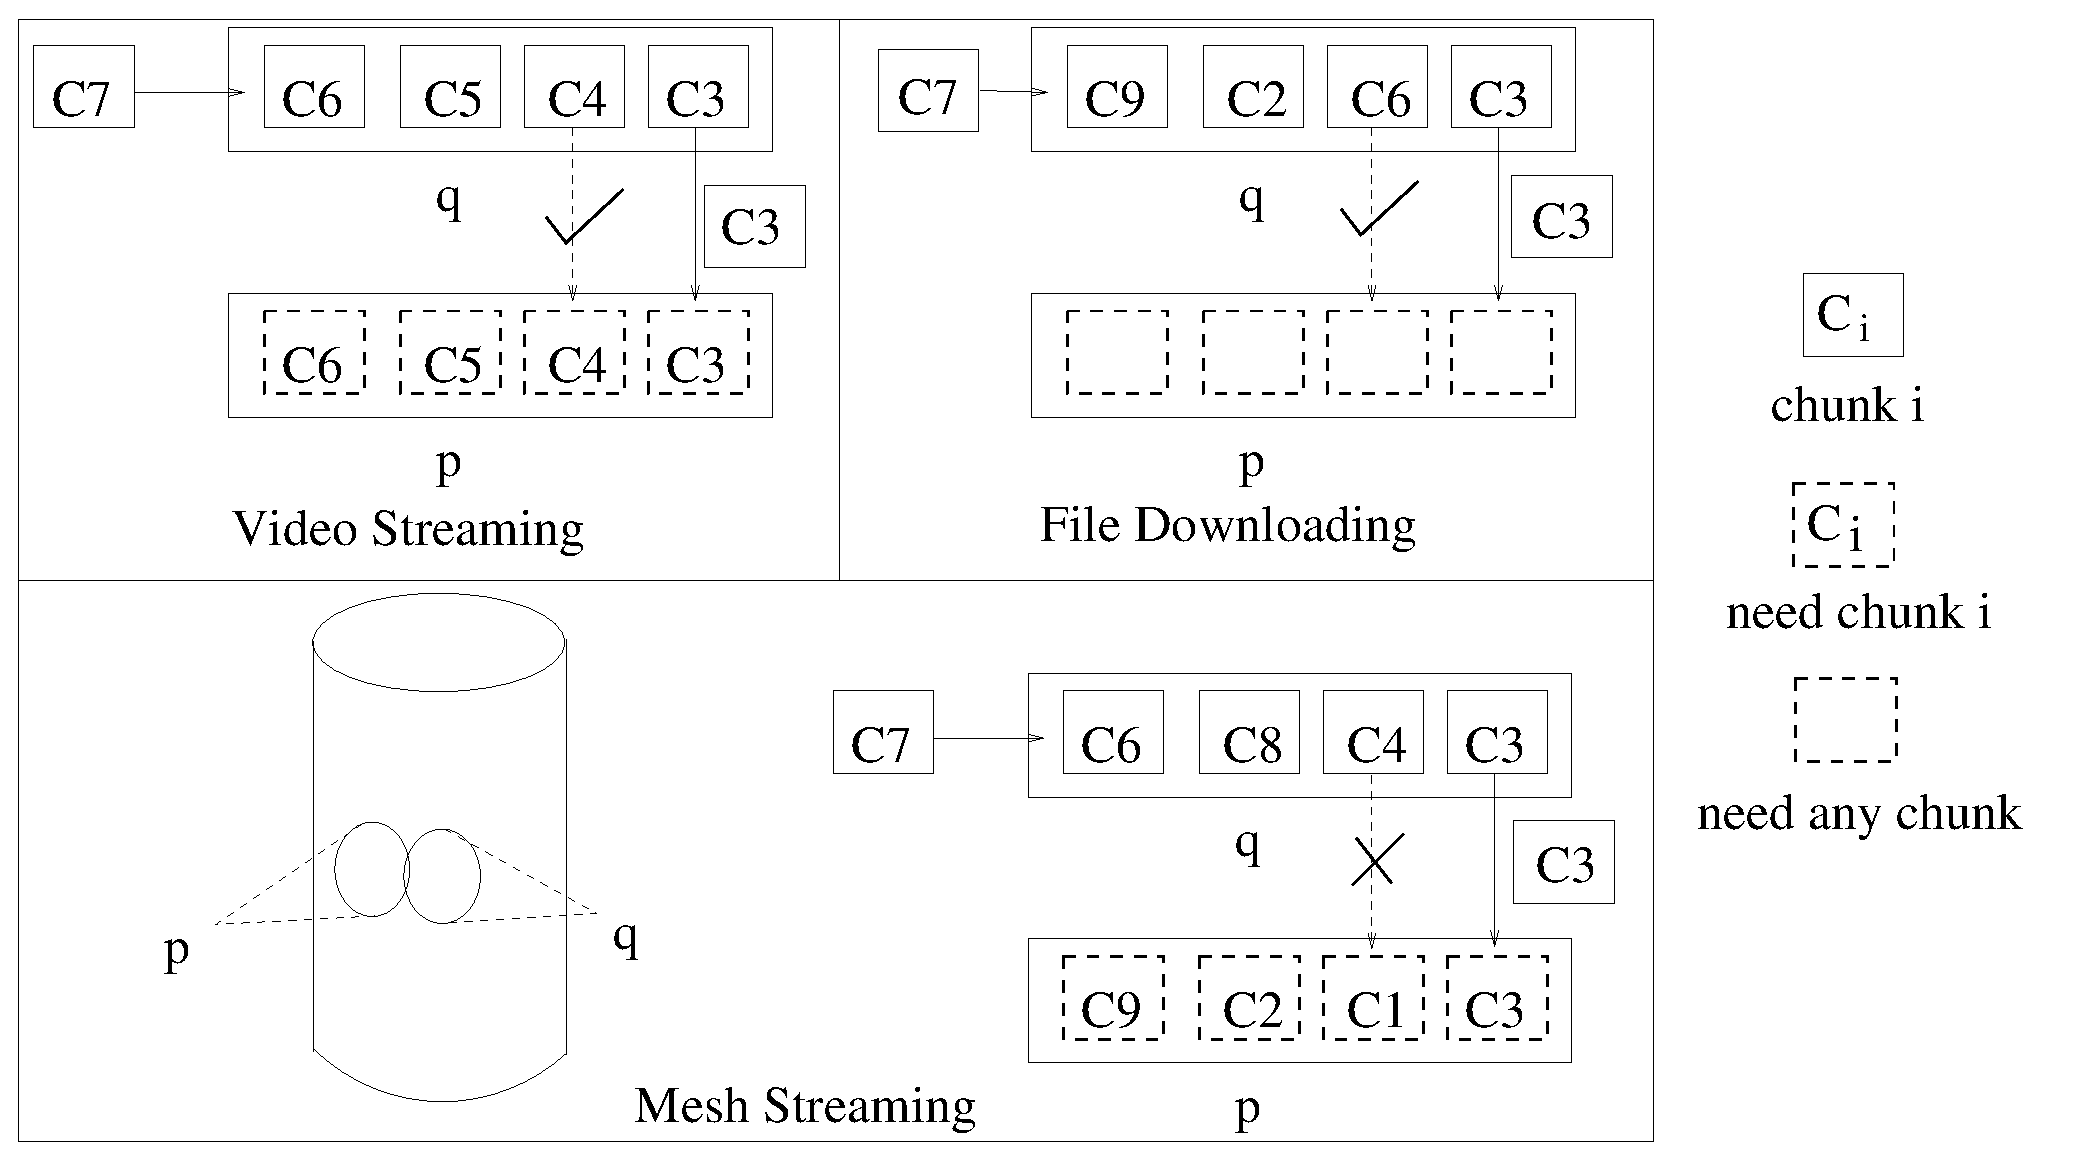
\epsfig{file =diff.eps, height = 2.5in}
    \caption[Difference between P2P video streaming, P2P file sharing, and P2P view-dependent mesh streaming.]
    {In video streaming, peers receive chunks in the same order, so $p$
    may request many chunks from $q$ (e.g, in the order of C3, C4, C5).
	 In file sharing, peers can receive
    chunks in any order, so $p$ can request all chunks received by $q$
	(e.g., in the arbitrary order of C3, C6, C2). In
    P2P mesh streaming, however, a peer often needs to keep finding
    new providers.  If $p$ changes its view to be different from $q$,
	$q$ may not be able to supply $p$ with the needed chunks anymore 
	(e.g., C1). \label{f:diff}}
    \end{figure}

    Temporal locality does not apply to mesh.  In P2P mesh
    streaming, however, users might be interested in
    different parts of the mesh at different level of
    details.  Each may choose to look at different facets,
    or zoom into different levels.  Therefore, each peer may
    be interested in different chunks of the mesh at
    different time.  Consequently, even if peer $p$ can
    receive a chunk from peer $q$ now, $p$ may not receive
    subsequent chunks from $q$ later, since $p$ may request
    a chunk that $q$ has never seen and is not visible to
    $q$. %(See Figure \ref{f:diff}).  
    Thus, a peer would have
    to continuously query for peers to retrieve the mesh
    data from, as the peer's view point and level of details
    change over time.  More queries are needed in mesh
    streaming than in file downloading or video streaming.
    Reducing such overhead is one of the main challenges of
    P2P mesh streaming.

    Another characteristic of mesh streaming is that the
    session length, i.e. how long a user stays in the
    system, is significantly shorter than that in file
    downloading and video streaming.  Users usually leave
    the system after viewing all the interesting parts of a
    mesh in several minutes.  Such short session time
    increases the churn rate and makes typical approaches to
    reduce query overhead inappropriate. To reduce the
    number of queries, a peer typically caches information
    about the chunks available in a provider for future
    requests.  High churn rate invalidates these cache
    information quickly.

    %TODO{transition here}
    %The issue of scaling 3D streaming to a large number of users has not
    P2P view-dependent mesh streaming remains a new topic because
    of the difference we stated above. 
    Some related studies exist, but they are not sufficient.
    %been sufficiently addressed.  
    %In our previous work, we focus on
    %reducing the computational overhead at the server \cite{Cheng2008}, by
    %shifting the burden of visibility computation from the sender to
    %the receiver.  
    Hu et al. \cite{Hu2008} and Cavagna et al. \cite{Cavagna2006} have considered using peer-to-peer architecture to stream a 3D scene
    to improve scalability.  Our work is similar in
    spirit, but we focus on streaming single, large,
    progressive mesh in a view-dependent manner, rather than a 3D scene,
    %. Streaming a single, highly detailed, progressive
    %mesh is different from streaming of a 3D scene,
    %The 3D scene streaming, however, is quite difference with the
    %streaming of single highly detailed progressive mesh targeted in this
    %paper. 
    where visibility decision is mainly done at the object level.
    %%could we remove the following sentences for simplicity? 
    The streaming
    of a single visible object, however, is still following a fixed
    pre-decided order independent of the user's view point. 
    The object level view-dependent system works well
    for scenes with many small objects but not for the
    scenarios we target,
    where %one or a few highly detailed 3D models are streamed.
    the data size of one object is already huge.  
    Streaming %large 
    progressive meshes needs 
    a much finer granularity for view dependency. 
    In this chapter, we study view-dependent streaming at 
    chunk level, which can be of much smaller size (can be as small as a packet) than an object.

Yang et al. \cite{viewcast:yang} proposed a view-dependent 
3D video streaming system, in which a set of gateways is used 
to disseminate the streams depending on the views of the receivers.
Similar to our goals, the technique aims to reduce the server 
overhead.  The number of gateways, however, is limited and the
gateways are assumed to be stable.  Further, 3D videos are not
progressive in nature. 


\begin{comment}
\section{Receiver-Driven Mesh Streaming}
\label{s:receiver}

To exposit our P2P view-dependent mesh streaming system, we first address
the question of the visibility determination.
Traditionally, view-dependent mesh streaming systems use sender-driven
protocols, in which the receiver sends the view point to the
sender.  The sender computes which vertex splits are visible
and sends the vertex splits in the decreasing order of the
visual contributions to the receiver.  The sender also
maintains the states of which vertex splits have been sent
for each receiver, to avoid sending duplicate data.  This
design is originally meant for client/server architecture.
In P2P mesh streaming, a peer plays the role of the sender.
This design is not desirable for P2P streaming for three
reasons.  First, computing the visibility and sorting the
vertex splits are expensive and may deter peers from
participating. Second, a peer might not have the complete
mesh so determining visibility may not be possible.
Finally, maintaining the receiver states requires
synchronization across multiple peers, since a peer might
retrieve data from multiple other peers.

We have previously \cite{Cheng2008} proposed a
receiver-driven protocol, in which a receiver determines the
visible vertices based on its own view point and explicitly
requests these vertex splits.  The sender, under this
protocol, is stateless and simply serves the requests.  We
adapt the protocol in this work, as its stateless server
design fits naturally into P2P mesh streaming.

The key question in designing the receiver-driven protocol
is how a receiver can determine the visible vertices when it
has not yet received the complete mesh.  In our proposal, 
we exploit the progressive nature of meshes and assume that 
if a vertex is visible, the vertex from which it is split is also
visible. Therefore,
we split visible vertices to refine the mesh.
Our experiments found that
we can approximate the visible vertices with negligible
errors using this rule of thumb \cite{Cheng2008}.

    %\begin{figure}
    %\centering
    %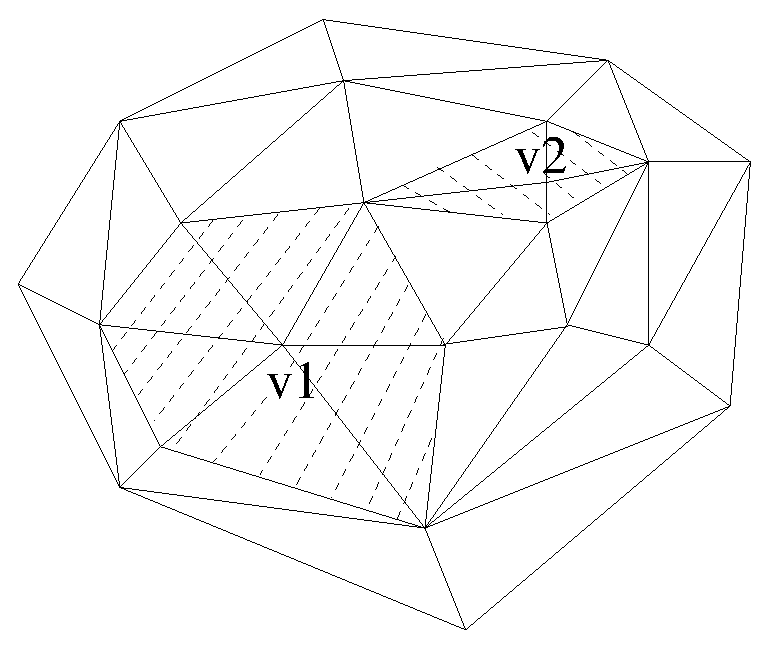
\epsfig{file =screen_area.eps, height = 1.0in}
    %\caption{%Screen area of two vertices: v1 and v2.
    %Rendered image on the receiver's screen. 
    %The shaded are the screen area of vertex $V_1$ and vertex $V_2$.
    %\label{screen_area}}
    %\end{figure}

    %The requesting order is periodically re-computed based on
    %the reconstructed mesh because new vertices are generated. 
    %Moreover, 
    %if the view point changes, the visual importance will
    %be re-computed and a new list of vertex splits will be requested.

    \begin{figure}
    \centering
    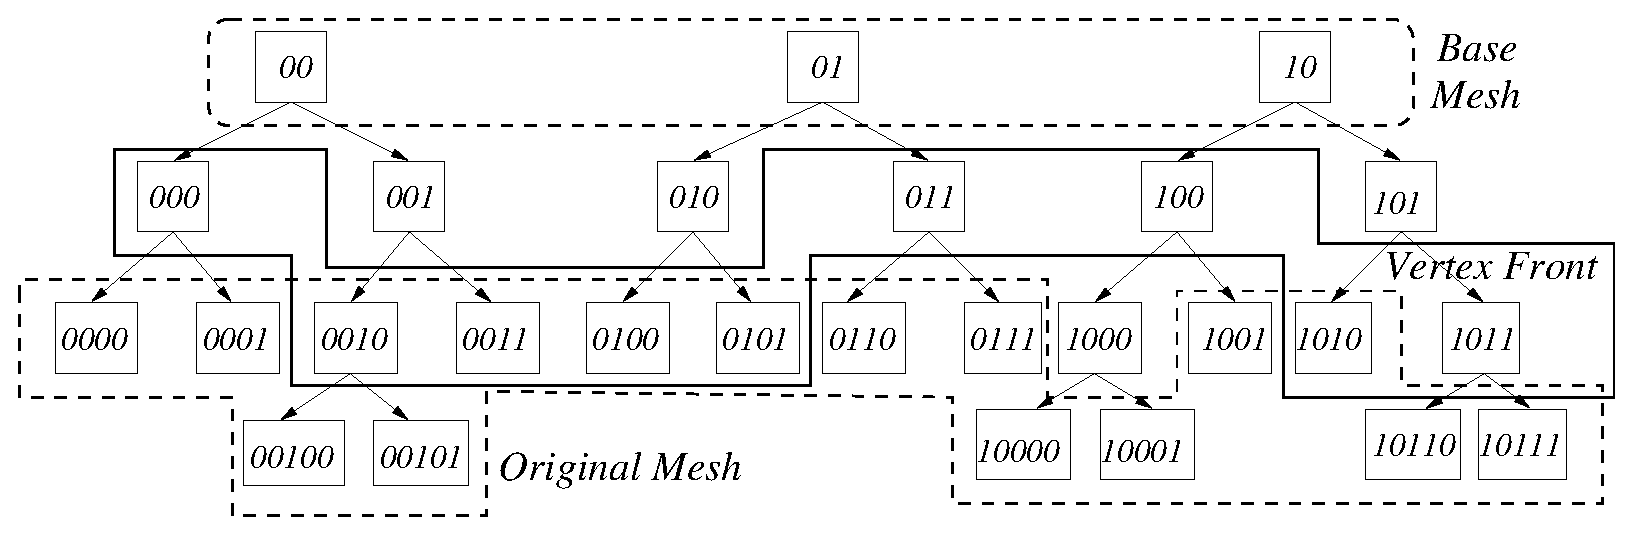
\epsfig{file = hierarchy.eps, height = 2.2in}
    \caption{Vertex hierarchy. A rectangle represents a vertex and the number inside
    is its identification number, including tree ID and node ID.\label{hierarchy}}
    \end{figure}
    Once a receiver finds a visible vertex, it
    requests the vertex split from the sender to split this vertex.
    To allow the receiver to explicitly request a vertex split, a
    unique identification (ID) is assigned to each vertex split.  In a
    progressive mesh, vertex splits are hierarchically organized as a forest of
    binary trees, 
    with a parent vertex $v$ being a coarser representation of its
    two children.  Thus, the leaves of the trees are vertices
    belonging to the original mesh (the mesh before simplification).  
    The roots of the trees are the 
    vertices in the base mesh (See Figure \ref{hierarchy}).
    
    We use the method proposed by Kim and Lee
    \cite{kim01truly} and assign each vertex a bit string
    consisting of two parts -- a tree ID and a node ID.  The
    tree ID is the sequence number of the root of this tree
    in the base mesh, and the node ID represents the path
    from the root to this vertex in the binary tree.  For
    example, if the tree ID is `01', which is also the ID of
    the root of this tree, the bit string `010' and
    `011' are the IDs of the left and right child of
    the root respectively.  Figure \ref{hierarchy} shows
    an example of vertex hierarchy.

    Since the IDs embed
    the vertex hierarchy, all IDs can be deduced.  The ID of the vertices in the base mesh
    is their sequence number, and the IDs of new
    vertices generated from a split can be deduced from the
    parent's ID.  Thus, the sender need not send additional information
    to identify a vertex.
\end{comment}

\section{Hierarchical Chunk Structure}
\label{s:chunk}
We now elaborate on how to group vertex splits into chunks while maintaining
progressiveness among the chunks.
    In the original design of receiver-driven protocol \cite{Cheng2008}, 
    the receiver explicitly requests individual vertex splits.
    Such design is not appropriate for P2P streaming for three reasons. 
    First, %since a packet can comprise
    %300 compressed vertex splits in our implementation, 
    %300 IDs need to be encoded in a request packet, equivalent to
    %600 bytes in our implementation. 
    the receiver needs to send one ID (2 bytes in our implementation)
    to request for one vertex split (less than 5 bytes in our
    implementation).
    Hence, the requests occupy a large proportion of the up-link bandwidth,
    which is precious in P2P streaming, in which the up-link bandwidth
    are needed to share data with other peers. 
    Second, data packets need to be generated dynamically at the
    sender whenever requests are received, increasing
    computation overhead and delay. 
    Finally, a peer needs to find proper
    peers to retrieve each vertex, which is expensive since the 
    number of vertices is huge in a large progressive mesh.

    To address these drawbacks, we adapted the receiver-driven
    protocol to the concept of chunk, commonly used in P2P systems.
    Our chunk, however, is of much finer granularity, to allow a peer
    the flexibility of retrieving only the %segments of mesh visible.
    mesh data within current visible region.
    Each chunk consists of multiple vertex splits, and each vertex
    split only belongs to one chunk. When a peer needs a vertex split,
    it finds the chunk that includes this vertex split and sends its
    chunk ID to request it. Each chunk is requested only once to avoid
    duplicate requests.
    %A peer sends a chunk ID to request a set of vertex splits.
    Once a chunk is received, 
    all the vertex splits in this chunk are decoded and processed.
    
    This method sacrifices some flexibility in choosing vertices,
    but has several advantages. First, 
    it significantly reduces the up-link bandwidth requirement since
    now only one chunk ID is needed to request a set of vertices.
    Second, the cost of searching for peers to retrieve data is also reduced.
    Third, grouping vertex splits into chunks can be done offline at
    the server, so no computation cost and time are needed by peers 
    for online packetization. 
    
    The question now is that how a peer knows which chunk to request
    when it decides to refine a certain part of a mesh.  
    One naive solution is to store the chunk ID together with vertex
    splits,
    but this method adds %additional data to a chunk 
    relatively expensive overhead to each vertex split. For example, the
    chunk ID usually accounts for 2 bytes, while each encoded vertex
    split accounts for only 3-4 bytes, so the overhead is more than 50\%.
    %(suppose the chunk
    %ID is 2 bytes and in our mesh encoding a vertex split just needs 3-4 bytes, the overhead is
    %more than 50\%).  
    Another method we considered is to organize the mesh into
    %a hierarchy of bounding boxes, and each bounding box is a chunk.
    many bounding boxes with the same size, and the vertex splits of the
    vertices inside a box belongs to a chunk. 
    The chunk ID can thus be deduced from the vertex coordinates.
    Nonetheless, this method still needs extra information to
    associate the chunks with the bounding box. %spatial cubes. 
    %Each packet needs to be assigned a spatial cell, such as a cube.   
    Moreover, since a
    vertex in a bounding box might have ancestors in other bounding
    boxes, this method increases dependencies among chunks, which might
    delay the decoding of some received vertices until other chunks are received.

    In our solution, we define chunks based on vertex dependencies as follows.
    First, we simplified the mesh to $s$ vertices. 
    For convenience, we choose $s$ to be the power of 2, i.e., $s = 2^i$.
    Then we split these vertices up to $w$ levels and use the 
    generated mesh as the base mesh. During the split, each of the
    original $s$ vertices is split to $2^w$ vertices. 
    Therefore, the base mesh has 
    %\begin{displaymath}
    $s \times 2^{w}  = 2^{i+w}$
    %\end{displaymath}
    vertices. 
    We divide these vertices into $s$ chunks and let the vertices
    split from a common ancestor to be in the same chunk.
    %and then we have $s$ packs. 
    For each of these vertices, we also add its descendants up
    to $d$ levels.  Thus, a chunk comprises of $2^w$ subtrees of
    vertices, each of height $d$.
    The vertices in a chunk satisfy the following
    conditions: (i) their vertex IDs (binary form) have a common
    $i$-bit prefix; (ii) the bit length of their vertex IDs is in $[i+1, i+d]$. 

    Therefore,  
    $s$ chunks are available to be requested when only the base mesh is received, 
    and each chunk has
    %\begin{displaymath}
    $2^{w} \times (2^{d} - 1)$
    %\end{displaymath}
    vertex splits.
    When a chunk is decoded,  $2^{w+d}$
    %\begin{displaymath}
    %$2^{w} \times 2^{d} = 2^{w+d}$
    %\end{displaymath}
    vertices will be generated. 
    
    We generate $2^d$ chunks from these $2^{w+d}$ vertices 
    by putting the vertices which only differ in the last $w$ bits
    into a chunk. These vertices are the roots of the subtrees in the chunk.
    Then, again for each vertex, we put its descendants up to $d$
    levels
    in the same chunk.  Therefore, we now have a chunk hierarchy with $2^{w}$
    root chunks and each chunk has $2^{d}$ children chunks.
    We call this chunk the 
    \textit{parent} chunk of these $2^{d}$ children.
    
    All vertices in a chunk have a common ancestor, so we 
    assign the vertex ID of this common ancestor as the chunk
    ID of this chunk (e.g. in Figure \ref{f:packetize}, the vertices
    in a chunk '000' are all children of vertex '000').
    In other words, the chunk ID is the longest common prefix
    of the binary form of the vertex IDs of its members.

   \begin{figure}[t]
    \centering
    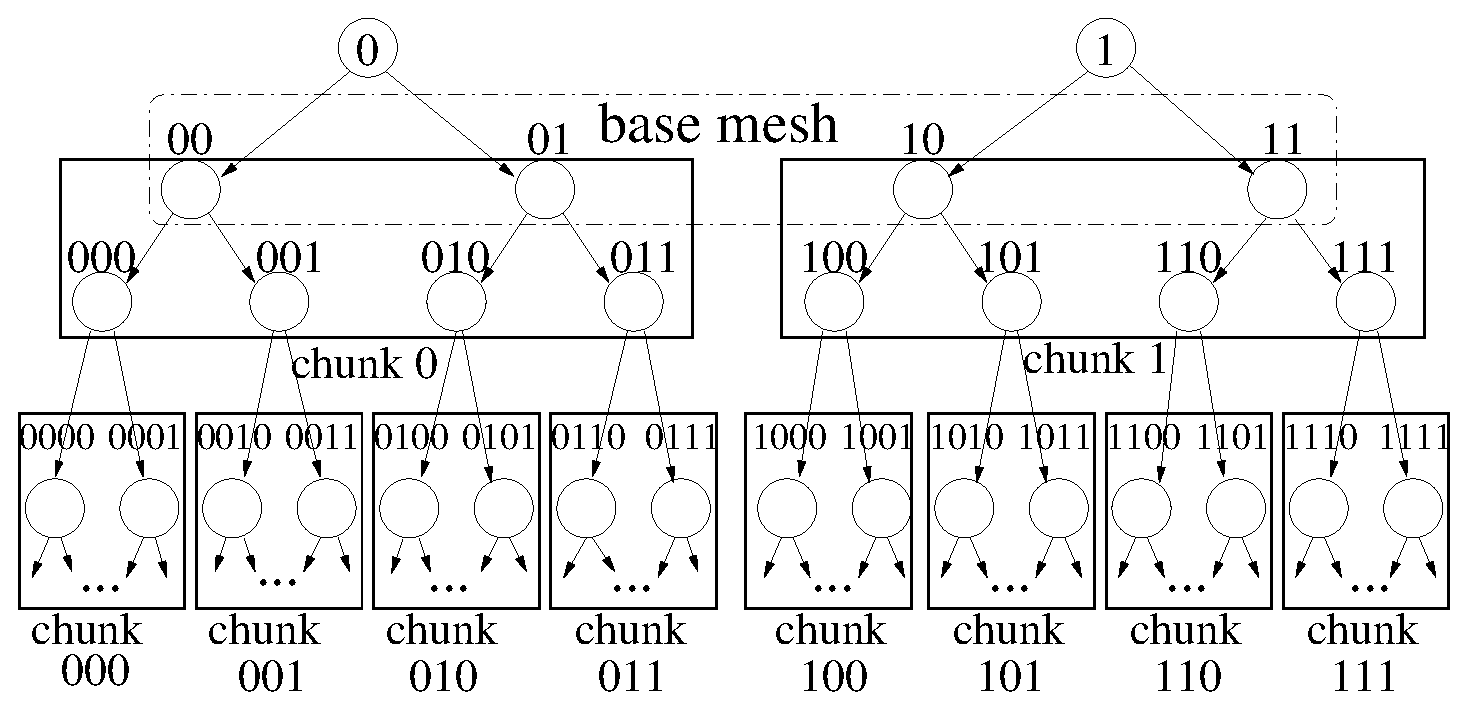
\epsfig{file = packetize.eps, height = 2.2in}
    \caption{An example of hierarchical chunk structure. Here $w$ = 1 , $d$ = 2
    and $i$ = 1. 
    \label{f:packetize}}
    \end{figure}
    Figure \ref{f:packetize} is a simple example with 
    $i=1$, $w = 1$, and $d = 2$. The base mesh has 4 vertices: 
    $00$, $01$, $10$ and $11$. 
    After the base mesh is received, two chunks $0$ and $1$ become
    available. 
    %and their packet ID are $0$ and $1$. 
    %forming the top group. 
    The vertex splits for vertices $00$ and $01$, as well as vertices from $000$ to $011$ 
    are inside the chunk $0$. 
    When chunk $0$ is decoded, %and all the vertex splits are processed, 
    eight new vertices from $0000$ to $0111$ are generated. 
    They become the root vertices of four new chunks from chunk $000$ to 
    chunk $011$.%, and these 4 chunks are in group $0$.  
    
    The main advantage of hierarchical chunk structure %grouping 
    is that it fits the dependencies among the vertex splits
    well.
    First, such packetization does not increase the dependencies
    among chunks because 
    %the  vertices in the chunks 
    %are independent to others.
    vertices in a chunk are independent of any vertex splits except
    those inside the ancestor chunks.
    Second, both the dependency among chunk IDs and the relation between
    chunk ID and vertex ID are implicitly 
    coded with the vertex ID.  
    If the vertex ID of the root vertex is $I_v$, 
    then the chunk ID is
    %\begin{displaymath}
    $I_c = (I_v >> d)$, 
    %\end{displaymath}
    %and the group ID is
    and the ID of the parent chunk is
    %\begin{displaymath}
    $I_p = (I_c >> d) = (I_v >> 2d).$
    %\end{displaymath}
    Since the vertex ID itself can be deduced as introduced in
    Chapter \ref{c:rdstream}, we implement this hierarchical system without any extra cost.

    Moreover, since the vertices in a packet are all children of a
    common ancestor, they are connected and are typically close to
    each other. Therefore, if one of the root vertices is needed by a
    peer, other root vertices are likely needed as well. Hence,
    it is reasonable to put them into one chunk.
    
    With this packetization, a peer that needs some vertex splits,
    can deduce the IDs of the chunks to
    request from the vertex IDs. Some invisible vertex splits may be received, but 
    because vertices inside a chunk are nearby each other, 
    they may be visible soon anyway when this peer changes viewpoint. 
    
    We now describe how to determine the values of $i$, $w$ and $d$.
    %A chunk has $2^{w}$ root vertices and each root
    %vertex has $2^{d} - 1$ children. 
    Suppose a chunk can carry about $n$ vertex splits after compression. 
    Therefore we have  
    \begin{displaymath}
    2^{w} \times (2^{d} - 1) < n 
    \end{displaymath}
    Choosing a large $w$ can improve the quality more quickly since 
    typically the vertex splits in low levels contribute more
    to the mesh quality,
    but it increases the possibility of including many invisible
    vertices.
    In our implementation, each chunk is the size of one packet, although we can easily generalized to larger chunk.  Since about 300 vertices can fit into an IP packet 
    (i.e. $n=300$),
    We choose $w=4$ and $d=4$, so a total of $240$ vertex splits are 
    in one chunk (if the progressive mesh is completely balanced).

    After deciding the value $w$, value of $i$ can be decided 
    based on the size of base mesh. 
    Certain number of vertices are needed in the base mesh to ensure 
    the minimal quality, and we know that the base mesh has $i \times 2^{w}$ vertices.
    So we can choose a proper $i$ value to satisfy the quality
    of base mesh. 
    In our implementation, we choose $i= 1024$. 
    Thus, the base mesh has
    $16382$ vertices.
%\subsection{Comparison}
%\todo{Then what is the cost of P2P: query, reliability}
%
%\todo{Why traditional decentralized P2P is not appropriate.}
%
%\todo{Why centralized method is a natural choice. High churn rate,
%small query size.}
%
%In this section, we introduce the problem of P2P mesh streaming, and
%compare it to other P2P systems, in particular, P2P file downloading
%and P2P video streaming.
%
%First, let us consider the design goals of a P2P mesh streaming
%system.
%The motivation of building a P2P mesh streaming system, like many
%other P2P systems, is to reduce server bandwidth bottleneck and
%infrastructural costs.  Thus, in any effective solution to this
%problem, a peer should, as much as possible, retrieves data from
%another peer and avoid getting data from the server.  
%
%Mesh streaming, unlike video streaming and file downloading, is highly
%interactive.  A user has the flexibility of changing its view point --
%she can zoom in, zoom out, or rotate around the mesh to view different
%regions of the mesh.  The response time, i.e., time between a user
%changing its view point, to seeing changes in the mesh displayed, needs
%to be as small as possible. 
%/todo{Note that even delay is large, the user can still see the
%response immediately.}
%
%A third requirement in P2P mesh streaming is low message overhead.
%Peers need to periodically exchange information about which chunks of
%data they have or need.   These control overhead should be as low as
%possible.
%/todo{Not necessarily by exchanging. In our system and centralized system,
%the information of providers are managed by the leaders.}

%The three requirements above, low server overhead, low response time,
%and low message overhead, are in conflict with each others.  Finding
%proper trade-offs between these requirements is a challenge of P2P
%mesh streaming.  If we remove the low message overhead requirements,
%then the solution is trivial -- just flood information about the
%chunks that a peer possess to all other peers frequently.  A peer can 
%thus identify quickly and accurately who has which chunk, allowing a
%required chunk to be retrieved from another peer without going
%through the server unless necessary (e.g., in cases where no other

%peers has the chunk).   We therefore focus on reducing message
%overhead in this paper in the condition that the other two requirements
%are satisfied.

%We now discuss the challenge in keeping low message overhead in P2P
%mesh streaming, by contrasting the uniqueness of mesh streaming to P2P
%video streaming and file downloading.

%    In this section, we introduce why the techniques used in P2P video streaming systems and P2P file sharing systems cannot
%    be directly used in P2P mesh streaming. The main difference is that in P2P mesh streaming, a client
%    has to keep finding a new peer as the source of data. 

%    Such need to switch frequently between peers to retrieve chunks from brings two difficulties 
%    in implementing a P2P mesh streaming system. First,
%    the message overhead for managing churns
%    and searching for chunks needed needs to be reduced with
%    careful design.  
%    As it is hard to retreive relevant chunks from the same
%    peer for a long time, the cost of searching for chunks cannot be amortized.
%    Due to the same reason, push-based methods
%    are not appropriate for P2P mesh streaming since it is not meaningful
%    to maintain an overlay when the peers do not remain connected
%    for long.
%    Second, the switching delay may increase the response time of the mesh
%    streaming system. Therefore, it is not realistic to use P2P
%    indexing and searching techniques with long delay, such as DHT, to
%    look for peers to retrieve relevant chunks from.
%    %peers as data sources because of the high delay. 
%    Ideally, 
    %The ideal case is 
%    each user knows a list of potential peers for a given chunk,
%    so that it can directly request data from one of these peers 
%    without searching.
%    \todo{Our system now does not ensure this ideal case.}
    
    %In brief, an effective P2P mesh streaming system has to help clients to find proper peers with short 
    %delay and meanwhile to keep the management cost low. 

%    One naive solution is to use a BitTorrent-like system, 
%    in which the mesh is divided into many small segments, each
%    corresponds to a chunk in BitTorrent.
%    A bit vector, like the piece graph in BitTorrent, can be used to indicate
%    whether a segment is available in a peer. 
%    This solution, however, does not consider view dependence and
%    progressiveness in mesh streaming.
%    First, the chunk needs to be small to ensure the flexibility needed in view-dependent streaming.
%    Hence the bit vector of a mesh might be huge. 
%    Second, dependencies exist among the data in a progresive mesh.
%    A chunk cannot be decoded before the chunks it depends on are
%    received. 
%    Therefore, a flat bit vector is not the most appropriate data
%    structure.

%    The realizations above motivate our design of P2P mesh streaming
%    system.  In our design, we employ a pull-based, receiver-driven protocol.
%    There is a set of challenges related to designing this protocol,
%    which we have addressed in our previous work \cite{Cheng2008}. 
%    We briefly present this protocol in the next section for
%    completeness.  We also design a hierarchical group system, which
%    hierarchically organizes chunks of a mesh, considering
%    the dependencies among the mesh data. The detail of this
%    organization is introduced in Section
%    \todo{totally changed.}
%    \ref{s:design}. 

\section{Content Discovery}
\label{s:content}

    We now consider how a peer can discover other peers can provide a given chunk.
    We first consider distributed
    hash table (DHT) and gossip-based techniques, 
    commonly used in file sharing and video streaming, and
    discuss why they are unsuitable for our application.  We then
    describe a simple centralized scheme that works reasonably well,
    followed by a more complex scheme that exploits the 
    hierarchical structure in the data, trading off
    the number of messages processed by server with response time and control overhead.

    DHT, a well-known technique for 
    content discovery,  hashes a chunk to a
    peer, which maintains a directory of peers storing the
    chunk.  DHT, however, is expensive to maintain and 
    causes huge control overhead under high churn 
    rate.  As mentioned, %we observed churning due to short session
    %time.  %DHT are expensive to maintain under high churn rate.
    short session time (typically several minutes)
    causes high churn rate in mesh streaming system.
    Moreover, DHT generally takes $O(\log{n})$ hops to lookup,
    too long for the application we have in mind.
    We therefore preclude DHT in our solution.

    Another common solution is gossip-based protocol, in which, peers
    exchange a bit-vector to notify each other which chunk it is
    holding on to. This approach is very flexible, but it does not fit
    well in P2P mesh streaming, either. The bit-vector is large
    due to small chunk size in our system, causing high
    control overhead. Second, due to short session times, much
    bandwidth is wasted in exchanging obsolete bit-vectors. 

    Compared to using DHT and gossip-based methods, maintaining 
    a centralized lookup directory at the server has two 
    advantages.  First, the lookup is only a single hop.  Further,
    the server can monitor peers' states and detect peer 
    failures more quickly than in decentralized P2P systems, 
    reducing the influence of churn.
    For these reasons, we study a P2P
    mesh streaming system with centralized lookup and evaluate its performance.

\subsection{P2P With Centralized Lookup}
\label{s:cp2p}

    We first consider one of the simplest ways of supporting content discovery,
    using a central lookup server that maintains the information of providers 
    for each chunk of the mesh. 
    The server maintains a list of peers who have downloaded each chunk.
    A peer $p$ who needs a chunk $i$ contacts the server.  The server
    chooses a peer who has chunk $i$ as provider and inform $p$ (see
    Figure \ref{f:cp2p} (a)).  Peer $p$
    informs the server after downloading chunk $i$, and is then added to the
    list of peers with chunk $i$.
    The server becomes the provider for a chunk $i$ when there is no 
    provider available for $i$ or when $p$ fails to receive a chunk from the
    given provider (e.g., if the provider has left or failed)
    (see Figure \ref{f:cp2p} (b)).

   \begin{figure}[t]
    \centering
    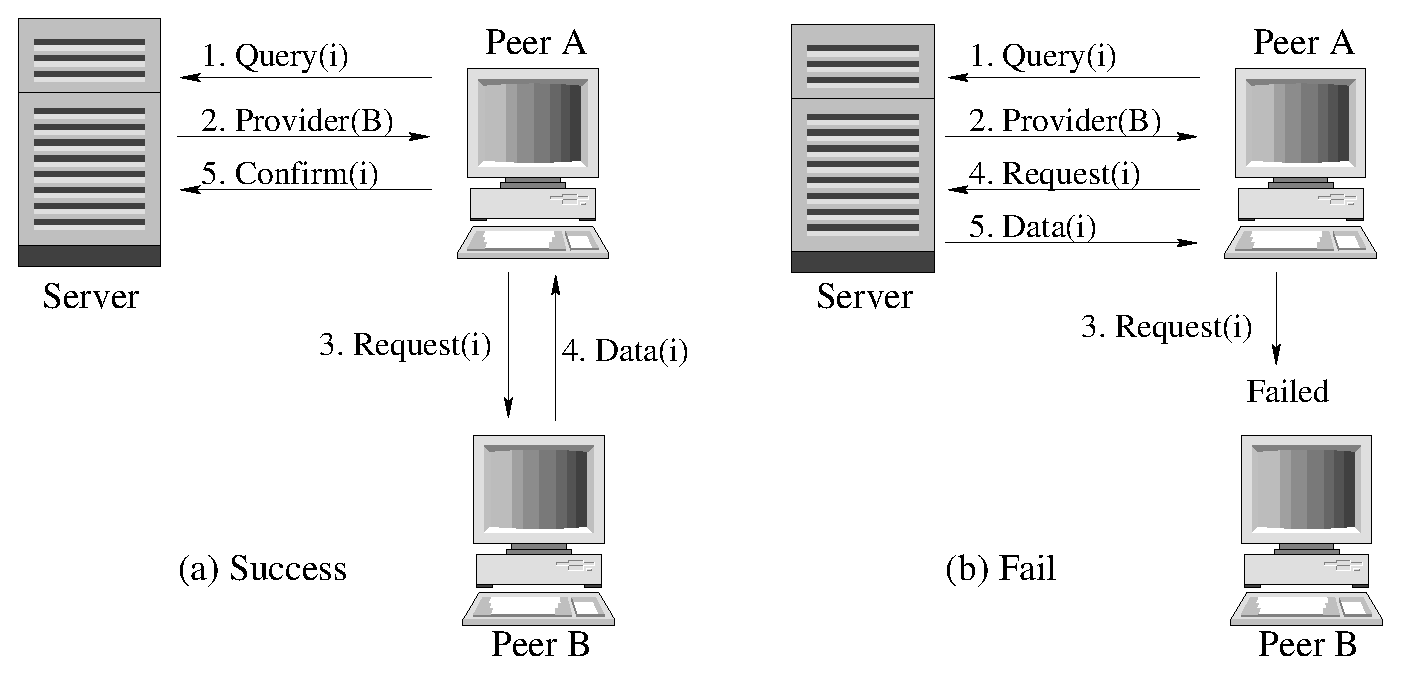
\epsfig{file = centralized.eps, height = 2.4in}
    \caption{Centralized Lookup. 
    \label{f:cp2p}}
    \end{figure}

    To keep the list of peers updated in an environment with high
    churn rate,  the server monitors
    the list of providers. %potential providers.
    In our implementation, peers periodically (every 5 seconds in our
    implementation) send
    heart beat messages to the server, and the server 
    ``forgets'' peers who have not been heard from after a certain
    period (15 seconds in our implementation).

    The centralized lookup is suitable for a small or middle-scale 
    P2P mesh streaming system.
    First, a query only costs two packets in terms of control overhead and 
    one RTT in terms of delay.
    Second, 
    states are maintained in one reliable
    node (the server), removing the needs of synchronizing states among
    peers. 
    Third, the server, maintaining all states, can employ better %simple 
    algorithms to determine the provider to improve the performance. 
    For example, topology-aware provider selection can 
    reduce the response time and inter-ISP traffic; load- and capability-aware 
	provider selection can balance the load among peers and improve fairness.
    
    Nonetheless, the centralized lookup is not scalable to large
    number of peers, as provider monitoring and selection incur
    server overhead.  Every request still causes a small packet to be
    sent from the server.  We only decrease the size of outgoing 
    packets, not the quantity.   When
    the cost in handling requests is expensive
    (e.g. when topology-aware provider selection and load balancing is considered), 
    the CPU becomes the bottleneck. 
    For example, for a server with 100Mbps outgoing bandwidth and four 2GHz
    %\todo{8 GHz is beyond today's technology?} 
    CPUs, assuming the outgoing packet size is 64 bytes, 
    then the transmission delay is only $4.92\mu{s}$. If 
    handling a request requires more than 40000 clock cycles, CPU becomes 
    the bottleneck rather than the network bandwidth. Therefore, to further increase the
    scalability, we have to reduce the number of requests and the
    cost in handling requests.
    
    To address this weakness, we propose a hierarchical P2P lookup approach,
    retaining most advantages of centralized lookup without 
    introducing much overhead.  We introduce this approach next.  

\subsection{Hierarchical P2P Lookup}
\label{s:hp2p}
    In our hierarchical P2P %mesh streaming system, 
    lookup approach, a set of
    peers, called a \textit{group}, is associated with each
    chunk of the mesh.  A group $G_i$ contains only peers
    that have already received chunk $i$.  Each group
    $G_i$ has a \textit{leader}, denoted $l_i$, which acts
    similarly to the server in the 
    %centralized P2P mesh streaming system we introduced
    P2P mesh streaming system with centralized P2P lookup we
    introduced
    above.  The members act as the providers for the chunk
    and are monitored by the leader.  Since the group and
    the chunk have a one-to-one mapping, the leader of group
    $G_i$ is also called the leader of chunk $i$.

    Assume for now that a peer knows the group leader $l_i$
    given $i$ (we will show how this is done later).  When a
    peer $p$ needs chunk $i$, it contacts $l_i$ to join
    group $G_i$.  The group leader $l_i$ then selects a
    provider from the members of $G_i$ and informs $p$ of the
    identity of this provider.  The peer $p$ then contacts the
    provider for the chunk.  Once %the peer 
    $p$ receives the
    requested chunk from the provider, it informs $l_i$ and
    becomes a member of $G_i$.

    Group leader acts as a provider when no other member
    exists.  But, unlike the centralized lookup approach, %P2P system, 
    if peer $p$ fails to receive chunk $i$ from a provider, it requests
    the chunk from the server rather than the group leader.  The
    rationale here is that the server is more reliable than
    a group leader, so the response time can be guaranteed.

    Note that one peer can belong to multiple groups.  But a
    peer should not lead multiple groups
    simultaneously, (i) to ensure the peer has enough
    capacity to serve requests for one chunk, and (ii) to
    avoid a single peer failure affecting multiple
    groups.

    Because a leader is also a peer, neither reliable nor
    having a well-known, fixed, address, two questions need
    to be answered: (i) how each peer knows the leader of a
    given group; (ii) how to deal with the leader failure.
    We explain our solutions in following sections.

    \subsubsection{Leader Hierarchy}
    %\begin{figure}[t]
    %\centering
    %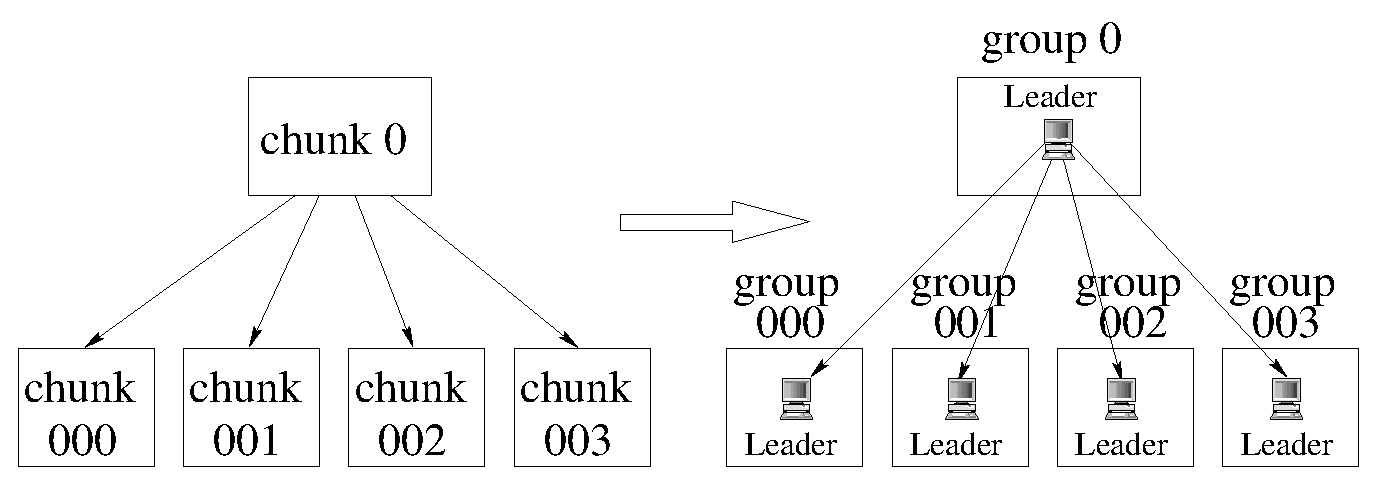
\epsfig{file = leader_hierarchy.eps, height = 1.1in}
    %\caption{From chunk hierarchy to leader hierarchy. 
    %\label{f:leader_hierarchy}}
    %\end{figure}

    Leaders inherit the hierarchical structure of
    chunks, due to the one-to-one mapping
    between groups and chunks.  The leaders form a tree, 
    mirroring the structure of chunks.  We use the common terms 
    leaf, root, parent, and child to describe leaders and their 
    relationship in a self-explanatory way.  Further, 
    we consider the server as the parent of all root leaders.
    
    Due to the dependency among the chunks, children of a
    chunk $i$ is only useful after $i$ is received.  Hence,
    it is natural for a leader to supply the information of
    its children to its members.  When a peer joins the
    group $G_i$, in addition to the information of provider
    $s_i$, the leader $l_i$ also returns the information of its children.
    By exploiting the hierarchical property of the chunks, the 
    leader information is obtained progressively without any query.

\subsubsection{Leader Assignment and Replacement}

    In this section, we explain how leaders are assigned and
    how a failed leader is replaced.
    Initially, no peer exists in the system, and the server
    behaves as the default leader of all chunks. When a
    non-leader peer $p$ joins a group $G_i$ led by the
    server, the server assigns $p$ as the leader of $G_i$.
    The server will not assign a peer as a leader if this
    peer is leading another group.
    When there are many candidates, how the server selects leaders
    is an interesting topic for further research. In our current
    implementation, the server only chooses peers with enough
    uploading bandwidth (larger than 512Kbps) as leaders.

    Since leader assignments and replacements are done by 
    the server, the server knows the current leader hierarchy.
    When assigning a peer $p$ as the leader of group $G_i$, the
    server also include information about $p$'s parent and 
    children in the tree.  The new leader then notifies its 
    parent and all its children of its new role.   

    \begin{figure}[t]
    \centering
    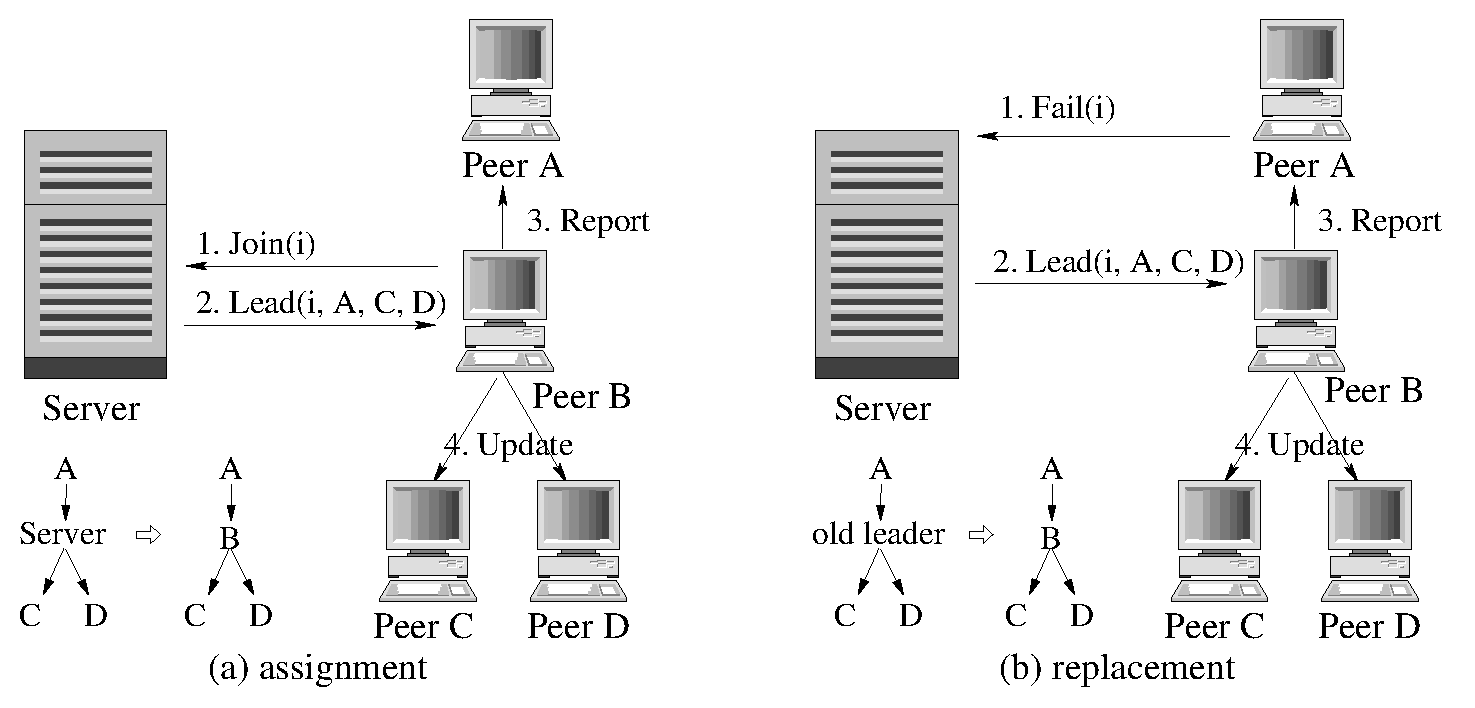
\epsfig{file = leader_assign.eps, height = 2.4in}
    \caption{(a) Peer B is assigned a leader. (b) An old leader is
    replaced by peer B. 
    \label{f:leader_assign}}
    \end{figure}

    To maintain the tree of leaders, a parent monitors all
    its children via heart beat messages.  Failure of a
    child is reported by the parent to the server, which
    then chooses one non-leader peer from the peers who
    newly joined the system (see Figure \ref{f:leader_assign}(b)).  
    The server maintains a list of recent, non-leader peers 
    who query the server for root leaders initially. 
    If no such peer is available, the server becomes the leader 
    itself.  
    
    The leader replacement information is disseminated
    %to all group members, parent, and children of the leader.
    to the parent and children of the leader when the new leader
    notifies its role. The parent leader in turn notifies
    its own members of this leader changes. So a member in the parent
    group of $G_i$ will always know the updated leader
    of $G_i$. 

    It is possible that a peer may contact a failed leader
    and experience timeout.  If a peer receives new leader
    updates from the server, it contacts the new leader;
    otherwise it requests the chunk from the server and 
    reports the failure.
    
\subsubsection{Reducing Monitoring Overhead}

    A peer becomes a member of group $i$ when it receives
    chunk $i$.  For a popular chunk $i$ (such as the root), 
    many members may exist.  Monitoring and maintaining 
    a large number of members is expensive for the leader.
    Furthermore, after receiving many chunks, a peer belongs
    to many groups, leading to high control overhead.
    This problem can be easily solved by restricting the 
    group size and the number of groups a peer belongs to.  

    We reduce the number of group a peer belongs to by the 
    following rule: if a peer $p$ obtained two chunks $i$
    and $j$, and $i$ is an ancestor of $j$, then $p$ only
    belongs to $G_j$.  

    By following the above rule, as a peer progressively 
    obtains more and more chunks, it joins groups that are
    lower down the hierarchy and leaves the higher groups.
    Note that a peer leaves a group as long as it obtains
    \textit{any} of the children chunks, not necessarily
    all.  At a later time, a peer may want to download a 
    child chunk $i$ of a group it has left (perhaps due to 
    a change of view point).  But, since a peer is no 
    longer in the parent group of the chunk $i$, it may not
    have up-to-date information about the leader of $i$.

    To avoid this, a group leader propagates updates %information 
    about its children down to its sub-tree.  As a result,
    a peer always knows its leader, the leader's ancestors,
    and the immediate children of the leader's ancestors.
    Knowing the children of the leader's ancestors allows
    a peer to download any children chunk through the leaders.

    This solution raises another problem.  If a peer belongs
    to multiple descendants of a group $G_i$, it may receive
    duplicate leader updates, %information, 
    leading to unnecessary messages.  
    Such duplicates can be removed by simply having
    this peer to explicitly register it to the leader closest
    %the peers to explicitly register themselves for updates.
    %If a peer belongs to multiple descendant groups of $G_i$, 
    %it registers to the leader closest 
    (in terms of hops count in the
    leader hierarchy) to $l_i$ for leader updates of $G_i$.
    This peer will not receive leader updates of $G_i$ from other
    leaders since leaders only send its members the messages they have
    registered. %to avoid 
    %Such duplicates can be removed by simply having the
    %peers to register themselves for updates from the leader
    %of a subset of groups.

    \begin{figure}[t]
    \centering
    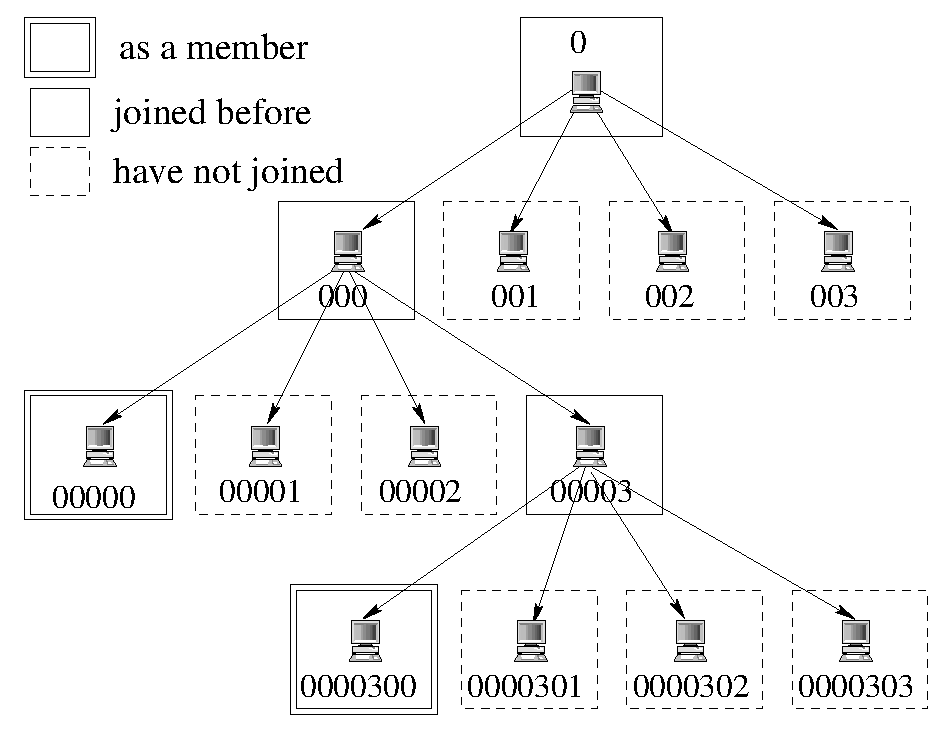
\epsfig{file = register.eps, height = 2.5in}
    \caption[Peer register in various groups.]
    {This peer will register in Group $00000$ for leader
    updates from group $0$
    and $000$, and it will register in Group $0000300$ for leader
    updates from group $00003$. 
    \label{f:register}}
    \end{figure}
    For example, as shown in Figure \ref{f:register}, a peer is a member in both group
    $00000$ and $0000300$. It has already received chunk $0$, $000$,
    and $00003$ before, but has left those groups. Since it
    may join group $001$, $002$, and $003$ in the future, it needs the
    leader updates from group $0$. Group $00000$ and $0000300$ are
    both descendant groups of group $0$, but $00000$ is closer to group
    $0$, so this peer registers to the leader of group $00000$ %that it needs the
    for updates from group $0$. 
    Similarly, it registers to the leader of 
    group $00000$ %that it needs 
    for updates from group $000$
    and registers to the leader of group $0000300$ %that it needs
    for updates
    from group $00003$. 
    This method ensures that the leader updates will be received with
    the minimum delay
    and without duplication.

    Note that only non-leader members may leave a group. To keep the leader
    hierarchy stable, the leader always stays in the group until
    it fails or the server assigns a new leader for this group.
    
    \subsubsection{Discussion}
    In the P2P system with hierarchical P2P lookup approach, %P2P system, 
    each group behaves like a small P2P system with centralized lookup
    approach. 
    First, most provider selection algorithms that can be used in centralized
    %P2P system, 
    lookup approach, 
    such as topology-aware and load balancing, can also
    be used in the hierarchical P2P lookup approach. %P2P system. 
    Second, providers are also monitored, so the failure rate of requests is 
    low even with high churn rate. Third,
    query for a provider can be finished within 1 RTT in
    most cases. In short, most of the advantages of the 
    %centralized P2P system are kept. 
    centralized lookup approach are retained.

    Compared with the centralized lookup approach, %P2P system, 
    the management overhead of the 
    server in hierarchical P2P lookup approach %P2P system 
    is significantly reduced. 
    In the stable stage, most group leaders are peers, so the server
    only monitors the leaders of the top chunks instead of all the peers in 
    centralized P2P system. 
    In addition, in hierarchical P2P lookup approach, %P2P system, 
    the server is also responsible
    for replacing the failed leaders, and thus maintains the leader hierarchy
    at a small overhead.
    First, the number of leaders only relates to
    the number of chunks and thus is independent of the number of peers. 
    Second, the rate of replacing leaders 
    only relates to the leaving rate of the peers, which is typically
    small compared with the total number of peers.
    Thus, the management overhead is significantly smaller and the
    server is more scalable to a large number of peers compared
    with the centralized lookup approach. %P2P system.
    
    The hierarchical P2P lookup approach, %system, 
    however, increases the control overhead and response time. 
    It may also cause more chunks to be provided by the server.
    First, more control messages are needed to maintain the leader
    hierarchy, to propagate leader updates down to sub-trees, and
    to exchange heart beat messages between parent and children. 
    Second, average response time increases since leaders may fail or leave.
    A peer who fails to contact a leader needs an additional RTT (to server) before receiving a chunk. 
    Third, leader failure causes the server to provide more chunks.
    Another reason is that some valid providers
    may not be used after they leave a group, 
    which will not happen in the centralized lookup
    approach. 

    In the next section, we further evaluate the centralized 
    and hierarchical P2P lookup approaches %P2P system 
    by simulations.

\section{Experimental Results}
\label{s:experiment}
    In this section, we present the experimental results to evaluate 
    the performance of the two lookup approaches we studied: 
    centralized lookup and hierarchical P2P lookup.

\subsection{Experiment Setup}

    We developed two systems to support the experiments:
    (i) a receiver-driven client and server 
    implementing view-dependent streaming
    of progressive meshes 
    used to collect and generate traces; 
    and (ii) a simulator that replays the traces generated
    and simulates large-scale P2P mesh streaming.

    The client-server system is programmed in C++ based on 
    OpenGL and OpenMesh\footnote{http://www.openmesh.org}. 
    In our experiments, we use the Thai Statue from  
    Stanford Computer Graphics Laboratory, %\footnote{http://www-graphics.stanford.edu/data/3Dscanrep/}, 
    which has 5 millions vertices and takes up 22.5 MB after
    being compressed with our encoding method. The mesh is packetized 
    into 147897 chunks following the approach introduced in Section
    \ref{s:chunk}.
    We choose this mesh since details exist all over the statue, 
    so users may have interest in different positions and levels of details 
    (see Figure \ref{thai}). 

    \begin{figure}
    \centering
    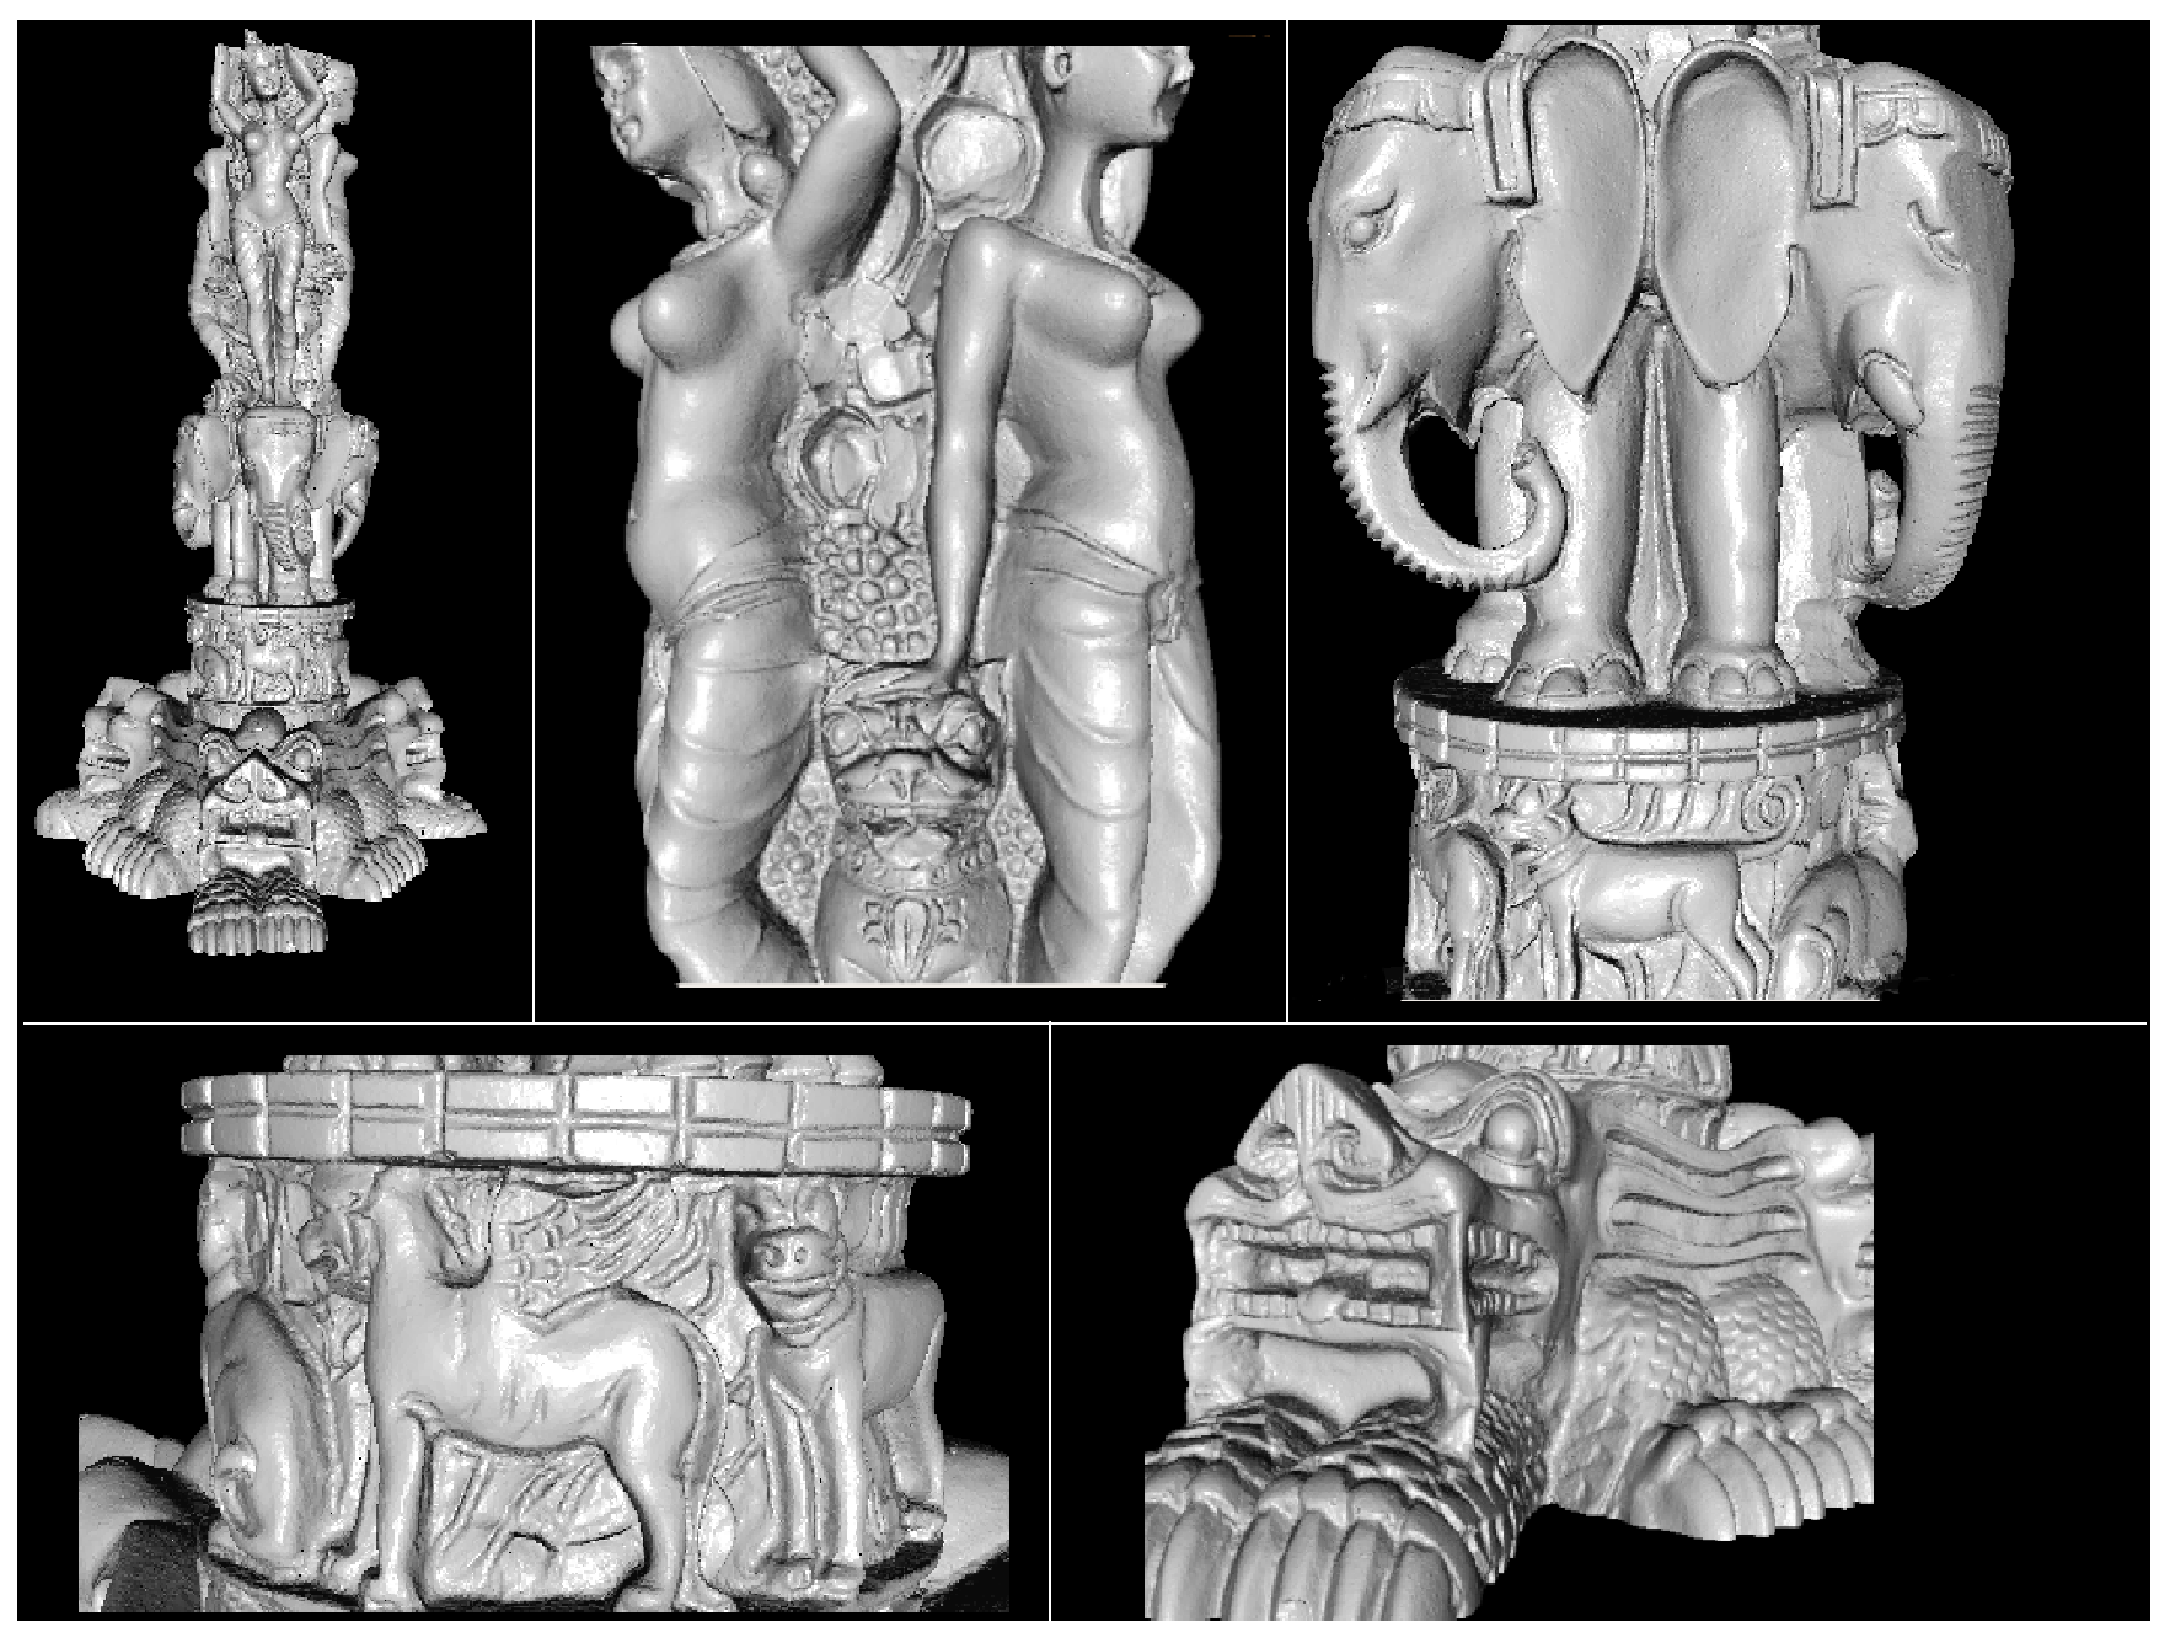
\epsfig{file =thai.eps, height = 3.5in}
    \caption[The Thai Statue]{%Screen area of two vertices: v1 and v2.
    The Thai Statue. The top left is the whole mesh, and the 
    rest is the closeup of some parts of it.
    Original mesh courtesy of Stanford Computer Graphics Laboratory.
    \label{thai}}
    \end{figure}

    %We collected 60 traces from 37 students from our
    %university.  The session length of these traces ranges
    %from 9 seconds to 380 seconds. When collecting the
    %traces, the streaming bandwidth is set to 320 Kbps, with
    %a client-server RTT of 400 millisecond.

    To simulate many users, we generated 6000
    synthetic traces following the model introduced in Section \ref{s:user:synthetic}.
    %after analyzing  
    %the collected user behavior traces, 
    %The session length follows a log-normal distribution
    %with $\mu = 18.23$, $\sigma = 0.754$ in $\mu$s. 
    %inter-action time interval (generalized extreme value distribution
    %with $\mu = 266,370$, $\sigma = 199,870$, and $\xi = 0.51$, in $\mu$s), 
    %and the probability of
    %selecting an action (zoom, pan, or rotate).
    We replay these generated
    traces to obtain the sequence of chunk requests
    and use the latter in the simulation.
\begin{figure*}[htb!]
\centering
\def\picheight{3.0in}
\begin{tabular}{c}
%\epsfig{file = plot/sessionLengthCDF.eps, height=\picheight, angle=270}
%\\
\epsfig{file = plot/delayCDF.eps, height=\picheight, angle=270}
\\
\epsfig{file = plot/bandwidthCDF.eps, height=\picheight, angle=270}
\\
\end{tabular}
\caption[CDF of the delay and bandwidth used in our simulation]
{CDF of peer-to-peer delay (mean =
75.8ms) and peer
bandwidth (download mean = 4292.8Kbps, upload mean = 1023.0Kbps) used in our simulation.
\label{f:cdf}}
\end{figure*}

    The P2P simulator is a discrete-event simulator based on 
    OMNeT++.  In our simulator, peers follow a Poisson arrival 
    model.  Each peer randomly selects a trace from 4000 random 
    traces we generated and leaves the system at the end of the trace. 
    Our experiment lasts for 320 seconds, and the period from $300s$
    to $320s$ is seemed as the stable stage (approximately).
    We choose the arrival rate ($\lambda$) as 20, 40, 60, and 80. 
    During the stable stage, the number of online peers are around 1974, 4030,
    6014, and 7974, respectively.


    %Figure \ref{f:peerNumber} shows the number of peers in the system
    %for different arrival rate ($\lambda$) of 20, 40, 60, and 80.

    %\begin{figure}[htbp!]
    %\centering
    %\epsfig{file=plot/numberOfPeers.eps, width=0.2\textwidth, angle =
    %270}
    %\caption{
    %The number of peers online corresponding to different arriving
    %rate.
    %\label{f:peerNumber}}
    %\end{figure}

    The end-to-end delay between two peers (including server to peers)
    are taken from the data collected from the Meridian
    \cite{meridian:wong}
    %\todo{CITE and check spelling of Meridian}.
    project. The original data is a $2500 \times 2500$ matrix
    recording the pair-wise delay between 2500 DNS servers. We assign
    each peer and the server a random DNS server and assume that the
    end-to-end delay of two peers equals the delay between their DNS servers
    (see Figure \ref{f:cdf}(a) for the CDF of end-to-end delay).

    The downloading and uploading bandwidth of peers are randomly
    selected from the data reported by DSLReports.com
    \footnote{http://www.dslreports.com/archive}, which records 
    and updates daily the
    access speed of users over the world. We use 21,206 samples, 
    collected on 14 April 2009.
    Figure \ref{f:cdf}(b) shows the CDF of the downlink and uplink
    bandwidth.

    In the following sections, we evaluate our P2P design in terms of
    server overhead, 
    incoming message rate of the server, 
    control overhead, and average response time.
    
    %Here, server overhead is %calculated 
    %defined as the ratio of the size of 
    %all data sent by the server to the size of mesh data received by
    %all peers, so for client-system system, the server overhead is
    %$1$.
    %Message overhead is the ratio of the size of message
    %data received to the size of mesh data 
    %received by all peers. 
    %The response time for each chunk request
    %is obtained by subtracting the receiving time of the chunk by the
    %sending time of the corresponding request. The average response
    %time is the average value of all the response times of chunk
    %requests during one second.

\subsection{Server Overhead}
\begin{figure*}[p!]
\centering
\def\picheight{3.0in}
\begin{tabular}{cc}
\epsfig{file = plot/serverdatarate.eps, height=\picheight, angle=270}
&
\epsfig{file = plot/serverDataRate_stable.eps, height=\picheight, angle=270}
\\
\epsfig{file = plot/serverOverhead.eps, height=\picheight, angle=270}
&
\epsfig{file = plot/serverOverhead_stable.eps, height=\picheight, angle=270}
\\
\epsfig{file = plot/serverVisit.eps, height=\picheight, angle=270}
&
\epsfig{file = plot/serverVisit_stable.eps, height=\picheight, angle=270}
\\
\end{tabular}
\caption[Comparison between centralized lookup approach and hierarchical
P2P lookup approach.]
{Comparison between centralized lookup approach and hierarchical
P2P lookup approach. The left column indicates how the results change with time, and
the right column how the results change with the arriving rate of
peers. The value in stable stage is averaged from $t = 300s$ to $t =
320s$.
%In the measurement, we choose the average value from 300 second
%to 320 second as the stable value.
\label{f:result}}
\end{figure*}

\begin{figure*}[p!]
\centering
\def\picheight{3.0in}
\begin{tabular}{cc}
\epsfig{file = plot/messageOverhead.eps, height=\picheight, angle=270}
&
\epsfig{file = plot/messageOverhead_stable.eps, height=\picheight, angle=270}
\\
\epsfig{file = plot/responseTime.eps, height=\picheight, angle=270}
&
\epsfig{file = plot/responseTime_stable.eps, height=\picheight, angle=270}
\\
\end{tabular}
\caption[Comparison between centralized lookup approach and hierarchical
P2P lookup approach.]
{Comparison between centralized lookup approach and hierarchical
P2P lookup approach. The left column indicates how the results change with time, and
the right column how the results change with the arriving rate of
peers. The value in stable stage is averaged from $t = 300s$ to $t =
320s$.
%In the measurement, we choose the average value from 300 second
%to 320 second as the stable value.
\label{f:result2}}
\end{figure*}
    In this section, we measure the server overhead in three forms. 
    First, we measure the outgoing data rate of the server.
    %, which is
    %the \emph{absolute server overhead}. 
    %In our experiments, when
    %$\lambda$ exceeds $40$, the absolute server overhead exceeds
    %1Gbps, which indicates client-server model cannot scale well without
    %increasing number of servers and outgoing bandwidth. Therefore,
    %we will not consider this model in the following experiments.
    Second, we measure the ratio of the server's outgoing data rate 
    to the total chunk size received by the peers. It is a \emph{relative
    server overhead} compared with the client-server model based
    system.
    Third, to evaluate how busy a server is in handling incoming messages,
    we measure the incoming message rate %the number of
    %incoming requests per second) 
    of the server to indicate the
    server overhead in handling incoming requests.

    The outgoing data rate is shown in  Figures \ref{f:result}(a) and
    (b).
    %, 
    %and relative server
    %overhead in Figures \ref{f:result}(c) and (d). 
    Figures \ref{f:result}(a) shows that the server outgoing data rate 
    in the client-server model exceeds 1Gbps when $\lambda$ exceeds $40$. 
    It indicates that the client-server model cannot scale well
    without increasing the number of servers and outgoing bandwidth,
    so we will not consider the client-server model in further
    comparisons.
    
    Figures \ref{f:result}(c) and (d) show the relative server
    overhead.
    The relative server overhead of the hierarchical P2P lookup is
    slightly larger than that of the centralized lookup in our
    implementation. The main reason is that more chunks are provided
    by the server in hierarchical P2P lookup than that in centralized
    lookup, as we will discuss in the section about response time.%The relative server overheadapproach
    %, so we could compare
    %our systems with the client-server model based system.
    %, so a client-server
    %system  

    %As we discussed, CPU may become the bottleneck under certain
    %condition. To evaluate how busy a server is, we measure the
    %number of messages per second 
    %incoming message rate of the server in both design. 
    The server incoming message rate of the two designs are shown in
    Figures \ref{f:result}(e) and (f), where we can see that 
    the hierarchical P2P lookup reduces the number of incoming
    messages by around
    80\%. Moreover, the incoming message rate increases more slowly with
    $\lambda$ in hierarchical P2P lookup, indicating that 
    the CPU overhead of the server (to handle the messages) also 
	increases more slowly.

    Note that in these two designs, the server responses to incoming
    requests are different. The responses are leader
    information (for failed \emph{join}s) and chunks (for failed
    \emph{request}s) in hierarchical P2P lookup approach, but are
    mainly provider information in centralized approach. 
    %is the leader information, while th
    %when using hierarchical P2P lookup, the server responses 
    %to the requests are data packets (chunks) and leader information, while the responses 
    %in centralized lookup includes also control information
    %(providers).  
    Retrieving a chunk or leader information is typically
    cheaper than deciding the best provider, especially when
    topology awareness and load balancing are considered. Hence 
    hierarchical P2P lookup not only reduces the incoming message rate, but
    also reduces the handling overhead per request to the server.
    
    %Although most of the packets sent by the server %\todo{by who?} 
    %are much larger in hierarchical P2P lookup approach,
    %but due to the less quantity, the outgoing data rate of the
    %server %'s \todo{?} outgoing data rate 
    %is only slightly higher 
    %to 
    %than that in centralized lookup as we see in previous section, 
    %especially when the number of peers are large. 

    \subsection{Control Overhead}
    %We measure the message overhead using $\frac{total data size - chunks
    %size}{total data size}$. 
    In this section we examine how much network bandwidth is used by
    control messages.
    We define control overhead as the ratio of the size of control
    messages to the size of chunks received by all peers during one
    second.
    Figures
    \ref{f:result2} (g) and (h) show that hierarchical P2P lookup has 
    higher control overhead than centralized lookup.
    The higher overhead is caused by maintaining the
    leader hierarchy and propagating leader updates. 
    %The small burst of control overhead along the curve is due to the 
    %periodic propagation leader updates.
    Moreover, in
    hierarchical P2P lookup, peers may belong to multiple %number of 
    groups, leading to more messages used in monitoring.
    Nonetheless, the control overhead of both systems are within an
    acceptable range. 
    
\subsection{Response Time}
    Another important metric to evaluate the P2P mesh streaming system
    is the response time. 
    The response time for each chunk request
    is obtained by subtracting the receiving time of the chunk by the
    sending time of the corresponding request.     Since %the 
    no strict order in receiving
    chunks is required in mesh streaming, the response time of a
    single request is not as important as that in audio and video
    streaming. Instead, we emphasize on the average response time of
    requests sent in a second, which is  %The average response
    %time is 
    the average value of all the response times of chunk requests in a
    second.

    Figures \ref{f:result2}(i) and (j) show that the hierarchical P2P system
    has higher average response time.
    The higher response time is caused mainly by two reasons.
    First, unlike providers, only one leader exists for one chunk.
    Leader failures cause many peers to spend one more round trip
    to obtain chunks. It is possible to use multiple leaders in a
    group in the future to reduce this effect. 
    Second, a leader in hierarchical P2P lookup approach does not have
    the information of all the providers as the server in centralized
    lookup, and congestion may happen due to limited supply ability,  %may cause congestion in the
    causing request failures and higher response time. %hence request failure.

    The response time of hierarchical P2P approach, however, is still
    under 1 second, which according to our experience, does not
    significantly affect users' experience.  When a user interacts with
    the mesh (e.g., rotate), the renderer responds almost immediately. 
    The response time of chunk requests only affects how fast the 
    mesh quality improves after users change their view points.
    
    %peers sending \emph{join}
    
    %messages to the failed leader. 
    
    %The difference in response time
    %between two designs, however, is small.  \todo{not small -- one is
    %twice the other!}
    %The reason is that the majority of requests are successful in both
    %systems, and the longer response time of small number of ``unfortunate''
    %peers does not change much. 

    \subsection{Summary}
    The results above indicate that
    both designs work well under an environment with heterogeneous peers, 
    asymmetric bandwidth, and high churn rate. Compared with a
    client-server design, the server outgoing bandwidth 
    is reduced by more than 90\%.  Hierarchical P2P
    lookup also reduces 60\% of incoming messages to the server,
    but generates  
    only around 10\% of control overhead when the number of peers is large. 
    The average response time of both systems is below 
    a second and does not affect the user experience due to the
    progressive rendering nature of the mesh.   
    Further, as the number of peers
    increases, the control overhead and response time remain
    relatively stable.

\section{Conclusion}
\label{s:conclude}
This chapter investigates into the problem of P2P view-dependent,
progressive mesh streaming, and studied two important components of
the problem - chunking and content discovery. We find that in P2P mesh
streaming, peers need to keep finding new chunk providers, increasing
the control overhead. Furthermore, the short session length of peers
increases the churn rate. We considered these unique characteristics
of mesh streaming and explored two content discovery schemes. We found
that centralized lookup works well with these challenges. To further
reduce the CPU overhead of the server, a hierarchical P2P lookup
approach can be used to move the lookup service to selected peers.

Further research can be done on other aspects of P2P mesh streaming. 
First, authentication is needed to detect malicious tampering of the
mesh by peers. Second, the user pattern in viewing the mesh could be
exploited for pre-fetching. We plan to pursue these research issues
next.


